\chapter[ANALYSE CONCEPTUELLE DU SYSTÈME D’INFORMATION]{ANALYSE CONCEPTUELLE DU SYSTÈME D’INFORMATION}
    \section[Introduction partielle]{Introduction partielle}
    Dans ce chapitre, nous allons présenter l’environnement professionnel dans lequel notre
    travail se déroule.
    \par
    Premièrement nous commençons d’abord par une brève présentation de Ngokaf Trans, puis nous introduisons
    la structure générale de son organisation avec ses différentes directions en particulier
    sa direction marketing pour qui notre projet est destiné, nous détaillons son organigramme ainsi
    que ses objectifs. 
    \par
    Et deuxièmement nous faisons une description du système d’information existant ainsi
    que du futur système d’information en ressortissant les besoins fonctionnels et non
    fonctionnels de ce dernier.
    \section[Environnement de travail]{Environnement de travail}
        \subsection[Présentation]{\textit{Présentation}}
        La société Ngokaf Trans est une compagnie de transport routier
        par bus de biens et de personnes, en République Démocratique du Congo
        et particulièrement dans les provinces du Haut-Katanga et du Lualaba.

        \subsection[Aperçu historique]{\textit{Aperçu historique}}
        La société Ngokaf Trans a été créée par Monsieur NGOIE KAFULA Didas,
        elle débute ses activités en 2020 dans le
        souci de rendre facile les déplacements de la population dans des conditions confortable
        dans les villes du sud de la République Démocratique du Congo.
        Rapidement la compagnie se développe et effectue des trajets, au départ
        entre Lubumbashi et Likasi, aujourd’hui entre Lubumbashi
        et Kolwezi. 

        \subsection[Situation géographique]{Situation géographique}
        Son siège social, se situe dans la province du Haut-Katanga, dans la ville de Lubumbashi,
        dans la commune de Lubumbashi sur croisement des avenues Moero et Kapenda.        

        \subsection[Objectifs sociaux]{Objectifs sociaux}
        La société Ngokaf Trans \acrshort{sarl} est une société commerciale,
        dont l’activité principale est :
        \par
        \begin{itemize}
            \setlength{\itemsep}{0pt}
            \item [\ding{226}] Le transport des personnes et des biens entres les différentes villes.
            \item [\ding{226}] Offrir les meilleurs services aux clients.
            \item [\ding{226}] Offrir des tarifs à bas prix permettent aux clients de voyager à travers les villes.
        \end{itemize}
        \subsection[Structure Organisationnelle]{Structure Organisationnelle}
            \subsubsection[Le Directeur Général]{Le Directeur Général}
            Le Directeur Générale planifie, dirige et supervise les activités reliées
            au transport, aux études d’élargissement, au rayonnement interne et externe
            de l’agence ainsi qu’à l’administration générale de la société.
            \par\noindent
            Le Directeur Générale de Ngokaf Trans s’assure également que les valeurs
            institutionnelles et les exigences de performances au sein de l’entreprise sont respectées.

            \subsubsection[Le Manager]{Le Manager}
            Le Manager est le représentant numéro un du Directeur,
            il a le rôle d’anticiper les risques, les tendances et les opportunités ; c’est lui décide
            et fait les choix stratégiques et tactiques. C’est lui qui recadre évalue les agents ;
            il a en même temps de rôle d’écouter, rédiger et présenter les feeds-back.
            Les problèmes cruciaux au sein de Ngokaf Trans sont résolus par le Manager,
            la fonction de fédérer et motiver et superviser toutes les agences lui reviennent.

            \subsubsection[Le Secrétaire de Direction]{Le Secrétaire de Direction}
            Le secrétariat de direction chez Ngokaf Trans est un bureau stratégique
            qui collabore directement avec le Manager il joue un rôle fondamental dans
            la bonne marche.
            \par\noindent
            Les compétences techniques du secrétariat de Direction chez Ngokaf Trans
            lui permettent d’organiser et d’encadrer le travail administratif dont il a la charge.

            \subsubsection[Le Responsable des Ressources Humaines]{Le Responsable des Ressources Humaines}
            Il a comme mission :
            \par
                \begin{itemize}
                    \setlength{\itemsep}{0pt}
                    \item [\ding{226}] Établir et contrôler les paies spécifiques ;
                    \item [\ding{226}] Tenir à jour les dossiers du personnel et remplir les obligations légales ;
                    \item [\ding{226}] Recruteur et intégrer le personnel.
                \end{itemize} 
            \subsubsection[Le Responsable Financier]{Le Responsable Financier}
            Il a comme mission :
            \par
                \begin{itemize}
                    \setlength{\itemsep}{0pt}
                    \item [\ding{226}] Contrôler la comptabilité de l’entreprise et la bonne
                    gestion de sa trésorerie, soit valider la rentabilité de l’entreprise ;
                    \item [\ding{226}] Valider la solvabilité de l’entreprise ;
                    \item [\ding{226}] Anticiper la stratégie de développement de l’entreprise
                    et les différents investissements et financement nécessaires.
                \end{itemize}
            \subsubsection[Le guichetier]{Le Guichetier}
            Il a comme mission :
            \par
                \begin{itemize}
                    \setlength{\itemsep}{0pt}
                    \item [\ding{226}] D’accueillir les clients dans le guichet  ;
                    \item [\ding{226}] De recevoir les commandes des clients ;
                    \item [\ding{226}] De vendre les tickets de bus.
                \end{itemize}
            \subsubsection[Le Contrôleur]{Le Contrôleur}
            Il a comme mission :
            \par
                \begin{itemize}
                    \setlength{\itemsep}{0pt}
                    \item [\ding{226}] De vérifier l’authenticité ou la validité des tickets de bus.
                \end{itemize}                
            \subsubsection[Le Responsable Informatique]{Le Responsable Informatique}
            Il a comme mission :
            \par
                \begin{itemize}
                    \setlength{\itemsep}{0pt}
                    \item [\ding{226}] Assure la disponibilité des différents équipements ;
                    \item [\ding{226}] Superviser l’achat des équipements informatiques ;
                \end{itemize}
\pagebreak        
        \subsection[Organigramme de l’entreprise]{Organigramme de l’entreprise}
            \begin{figure}[H]
                \centering
                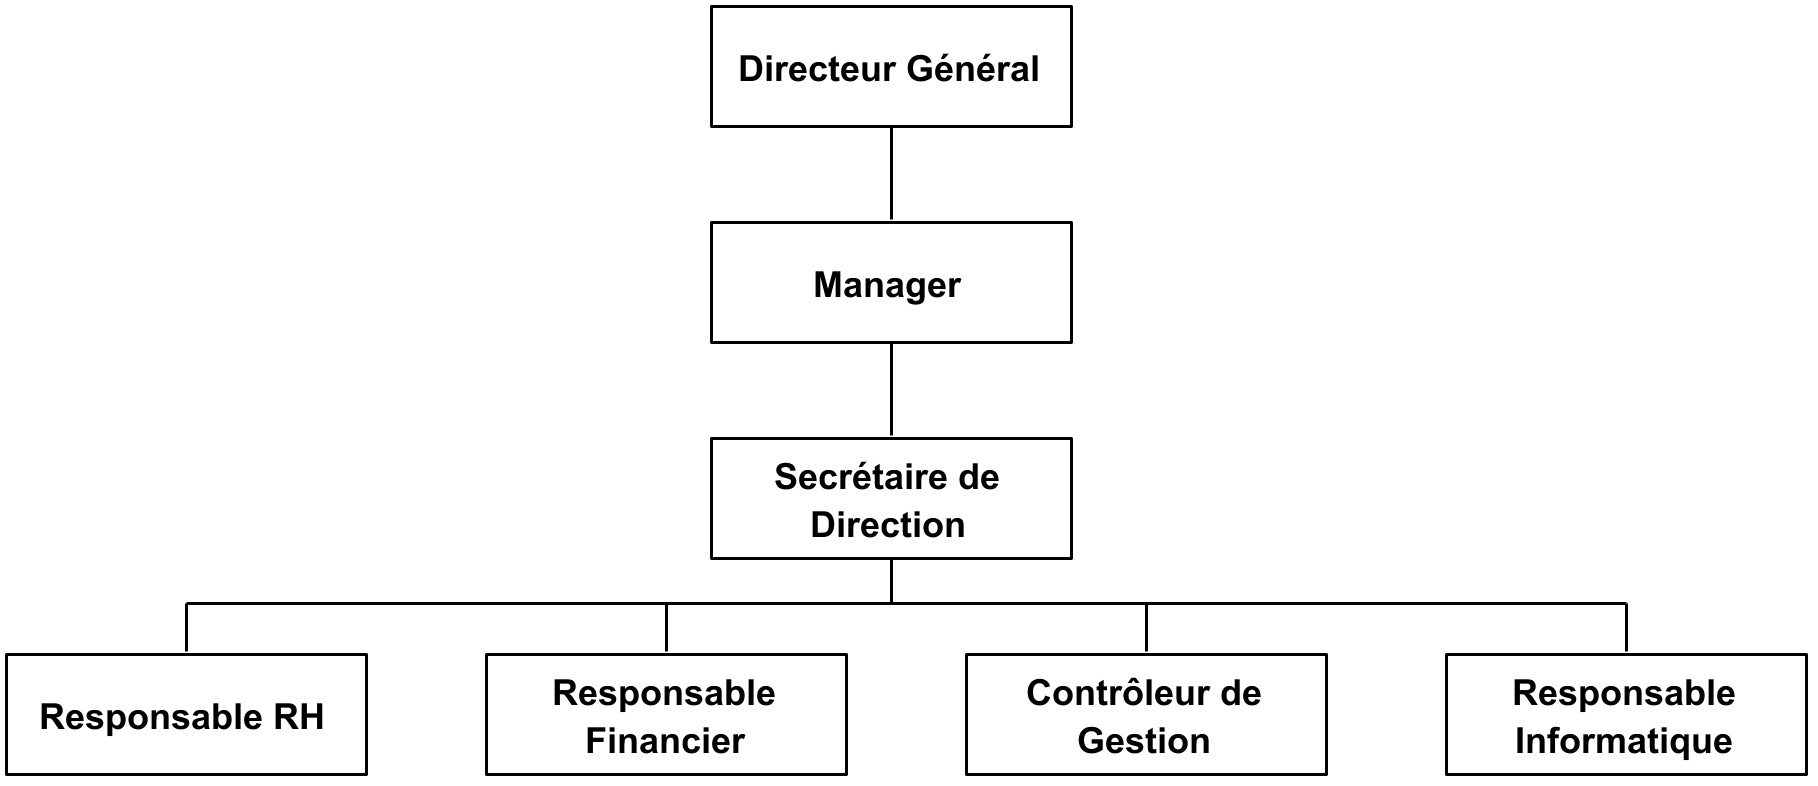
\includegraphics[width=120mm]{organigramme.png}
                \caption{Organigramme de la société Ngokaf Trans}
                \label{fig:Organigramme}
            \end{figure}
    \section[Analyse du système existant]{Analyse du système existant}
        \subsection[Diagramme de cas d’utilisation métier]{Diagramme de cas d’utilisation métier}
        \begin{figure}[H]
            \centering
            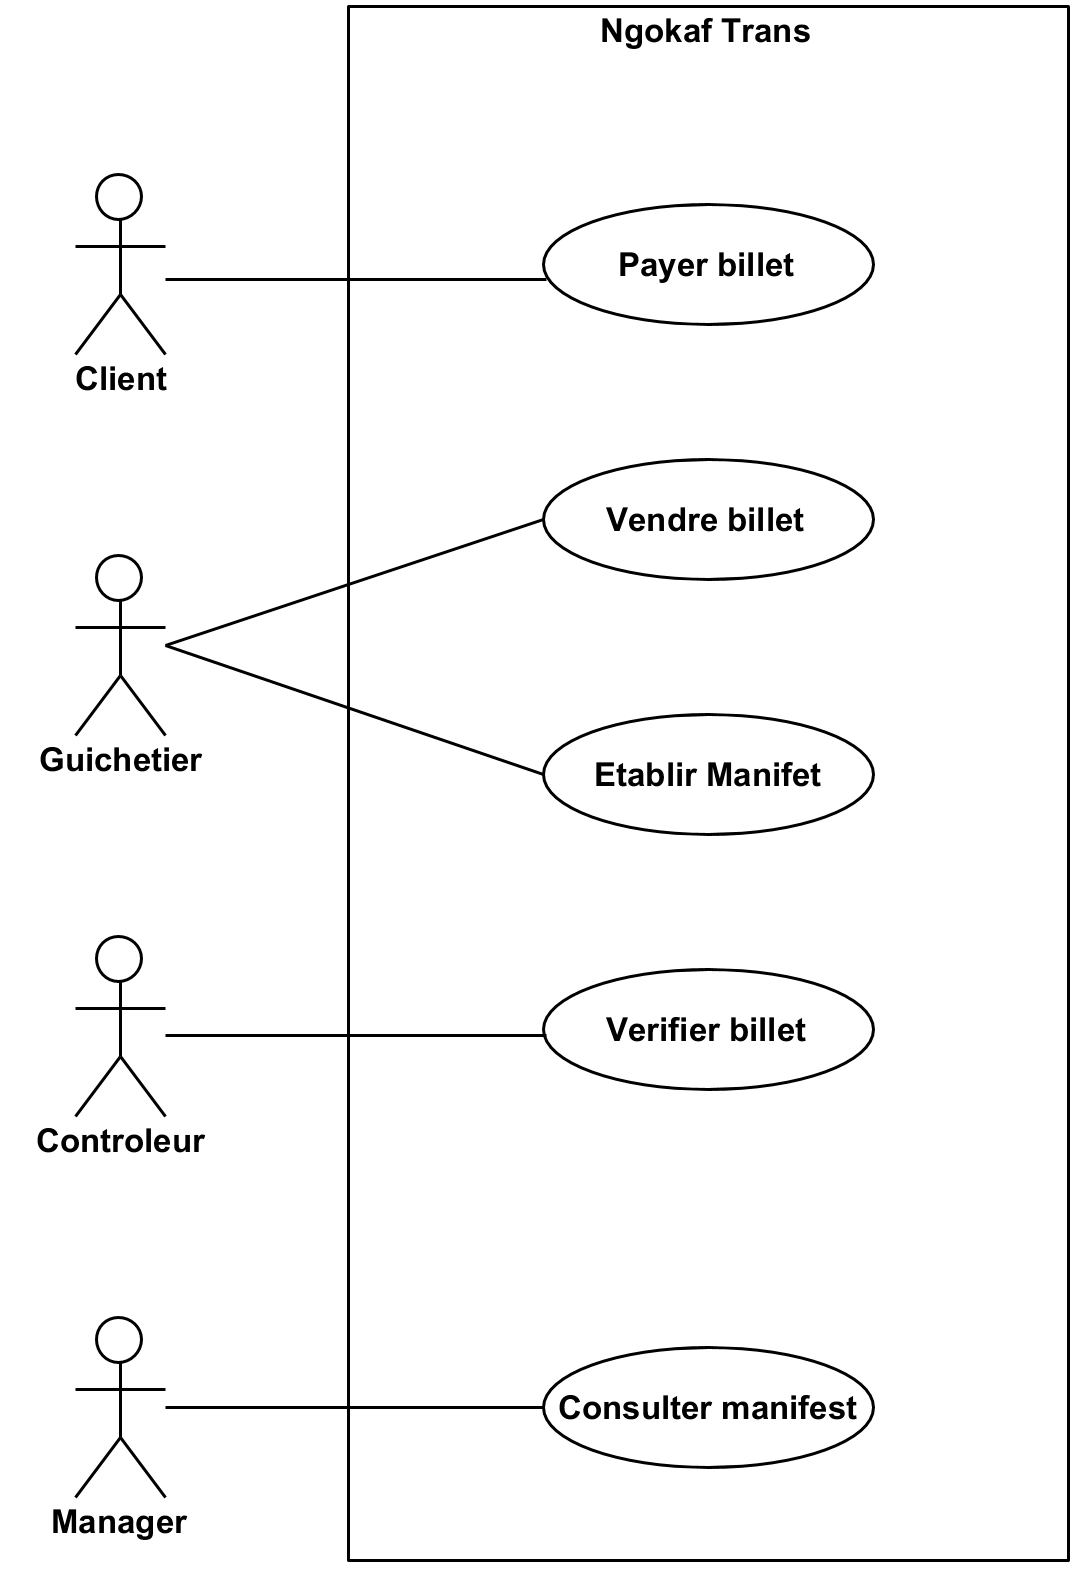
\includegraphics[width=75mm]{images/diagramme-de-cu/Systeme Existant.png}
            \caption{Diagramme de cas d’utilisation métier de Ngokaf Trans}
            \label{fig:DcuNgokaf}
        \end{figure}
\pagebreak
        \subsection[Diagramme d’activités métier]{Diagramme d’activités métier}
        Le diagramme d’activité fournit une vue d’ensemble du comportement d’un système en
        décrivant la séquence d’action d’un processus.
        \begin{figure}[H]
            \centering
            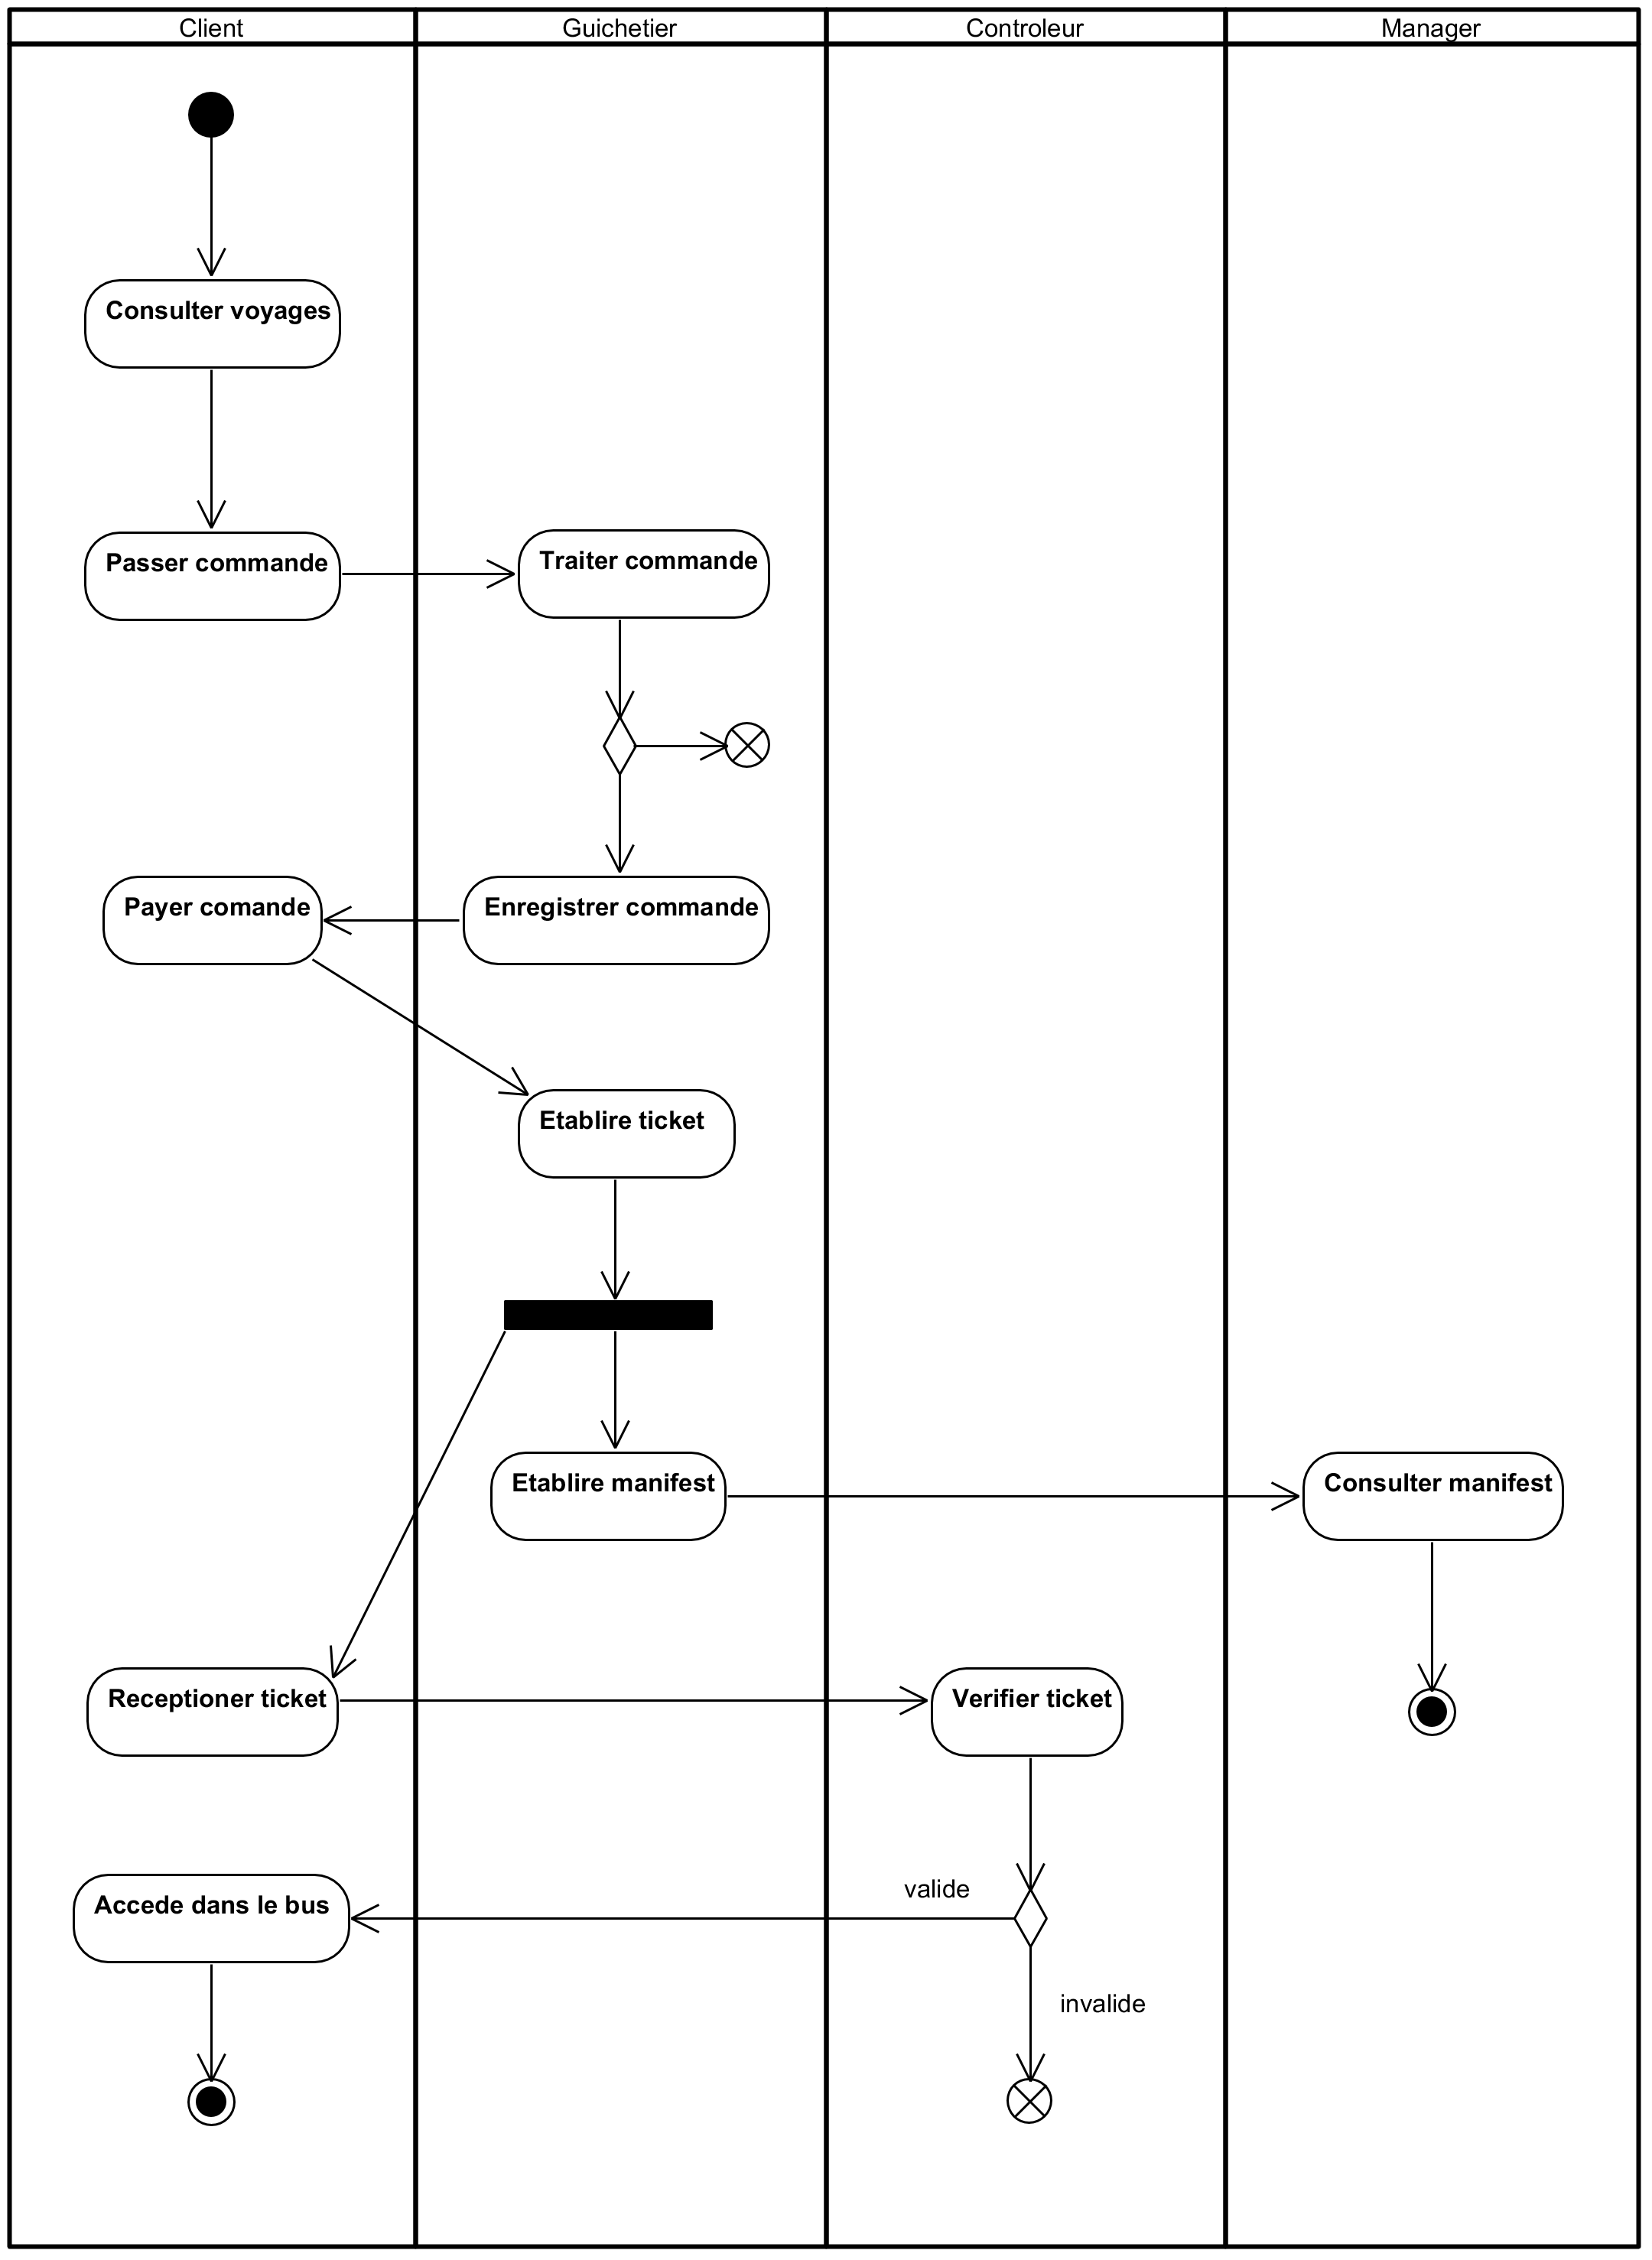
\includegraphics[width=140mm]{images/diagrammes-d-activites/metier Activity Diagram.png}
            \caption{Diagramme d’activités métier de Ngokaf Trans}
            \label{fig:DacNgokaf}
        \end{figure}
\pagebreak
        \subsection[Système de fidélisation existant]{Système de fidélisation existant}
        L’entreprise Ngokaf Trans ne dispose d’aucun système de fidélisation de son segment
        clients par conséquent les clients ne sont pas fidélisés. Néanmoins, il est important
        de noté qu’ils offraient. à leurs débuts, un calendrier à tous les nouveaux clients malheureusement
        sans savoir qui était le bon client (qui le méritait).
        \subsection[Système de prise de décision existant]{Système de prise de décision existant}
        Pour ce qui est de la prise de décision chez Ngokaf Trans, l’agent chargé des ventes
        envoie le rapport journalier au manager qui a son tour va prendre la décision sous deux
        aspects : s’il faut améliorer les services ou baisser le prix des billets.
    \section[Critique du système existant]{Critique du système existant}
    \par
    Les points faibles :
    \par
        \begin{itemize}
            \setlength{\itemsep}{0pt}
            \item [\ding{226}] Le manque d’une base de données
            \item [\ding{226}] La difficulté d’établir les rapports journaliers des opérations en un temps
            record par les agents.
            \item [\ding{226}] La difficulté de récolter les avis des clients. 
            \item [\ding{226}] Difficulté de définir les stratégies de fidélisation des clients.
            \item [\ding{226}] La difficulté de consulter les rapports des opérations à distance par le
            responsable de l’entreprise.
            \item [\ding{226}] La difficulté de prendre des décisions par manque de rapports de bonne
            qualité.
        \end{itemize}
    \par
    Les points fort :
    \par
        \begin{itemize}
            \setlength{\itemsep}{0pt}
            \item [\ding{226}] L’enregistrement de toutes les ventes grâce à Excel.
            \item [\ding{226}] L’établissement des rapports journaliers.
        \end{itemize}
    \section[Analyse des besoins]{Analyse des besoins}
    L’identification des besoins constitue la phase de départ de toute
    application à développer. Elle est l’étape dans laquelle nous allons identifier
    les besoins de notre application. Nous distinguons des besoins
    fonctionnels qui présentent les fonctionnalités attendues de notre
    application et les besoins non fonctionnels pour éviter le développement
    d’une application non satisfaisante ainsi de trouver un
    accord commun entre les spécialistes et les utilisateurs pour réussir le projet.
        \subsection{Besoins fonctionnels}
        Les besoins fonctionnels décrivent les exigences fonctionnelles
        des différents acteurs de l’application.
        \par
        \begin{itemize}
            \setlength{\itemsep}{0pt}
            \item [\ding{226}] \textbf{L’internaute} : il devra avoir la possibilité de voir
            les avis des clients et de créer un compte client. 
            \item [\ding{226}] \textbf{Le client} : il devra avoir la possibilité de
            donner son avis et de recevoir des offres ou messages promotionnels de la
            part de l’entreprise.
            \item [\ding{226}] \textbf{Le guichetier} : il devra pouvoir vendre les tickets
            de bus et ainsi récolter les données.
            \item [\ding{226}] \textbf{Le contrôleur} : il devra pouvoir vérifier l’authenticité
            du ticket du client. 
            \item [\ding{226}] \textbf{Le manager} : il devra avoir la possibilité 
            de consulter le rapport et de visualiser les graphiques des ventes et
            des avis clients. 
        \end{itemize}
        \par
        L’application doit pouvoir offrir à ses utilisateurs finaux les fonctionnalités suivantes :
        \subsection{Besoins non fonctionnels}
        Les besoins non fonctionnels sont les besoins qui ne sont pas des
        services rendus par le système, mais qui complètent les
        exigences fonctionnelles pour que la solution corresponde vraiment
        aux besoins des utilisateurs.
        \par
        En plus de besoins fonctionnels, l’application doit pouvoir avoir les qualités minimales
        suivantes :
        \begin{itemize}
            \setlength{\itemsep}{0pt}
            \item [\ding{226}] L’ergonomie.
            \item [\ding{226}] La fiabilité.
            \item [\ding{226}] La facilité d’utilisation.
            \item [\ding{226}] La robustesse et la sécurité.
        \end{itemize}
    \section[Solution proposée]{Solution proposée}
    Suite à notre analyse de l’existant, nous jugeons utile de mettre en place un
    système informatique qui devra premièrement, permettre la gestion de certaines activités
    de l’entreprise (la vente, la gestion du catalogue des voyages, le contrôle du ticket), deuxièmement
    permettre à l’entreprise de récolter les avis des clients, mais aussi d’évaluer les
    services proposés grâce à des questionnaires soumis aux clients, et pour finir, servir d’outil d’aide
    à la décision.
    \section[Conclusion partielle]{Conclusion partielle}
    Dans ce chapitre, nous avons procédé à la présentation de notre
    cadre de recherche qui est la société Ngokaf Trans. Nous avons étudié
    en détail le déroulement du processus, déniché les failles et les
    insuffisances dans le but de comprendre les problèmes rencontrés par la
    société Ngokaf Trans. Par la suite, nous avons identifié les besoins du
    point de vue de l’utilisateur qui est la société Ngokaf Trans, ainsi que
    les candidats, du point de vue technique en donnant une liste des exigences.
    \par
    Sur base de nos analyses, nous avons proposé une gestion de la clientèle et
    un système de prise de décision, concernant la fidélisation de la clientèle
    à l’aide d’une application informatisée. La connaissance de toutes les
    informations de notre analyse nous permettra dans le troisième chapitre
    de modéliser le nouveau système proposer.